% Options for packages loaded elsewhere
\PassOptionsToPackage{unicode}{hyperref}
\PassOptionsToPackage{hyphens}{url}
%
\documentclass[
]{article}
\usepackage{lmodern}
\usepackage{amssymb,amsmath}
\usepackage{ifxetex,ifluatex}
\ifnum 0\ifxetex 1\fi\ifluatex 1\fi=0 % if pdftex
  \usepackage[T1]{fontenc}
  \usepackage[utf8]{inputenc}
  \usepackage{textcomp} % provide euro and other symbols
\else % if luatex or xetex
  \usepackage{unicode-math}
  \defaultfontfeatures{Scale=MatchLowercase}
  \defaultfontfeatures[\rmfamily]{Ligatures=TeX,Scale=1}
\fi
% Use upquote if available, for straight quotes in verbatim environments
\IfFileExists{upquote.sty}{\usepackage{upquote}}{}
\IfFileExists{microtype.sty}{% use microtype if available
  \usepackage[]{microtype}
  \UseMicrotypeSet[protrusion]{basicmath} % disable protrusion for tt fonts
}{}
\makeatletter
\@ifundefined{KOMAClassName}{% if non-KOMA class
  \IfFileExists{parskip.sty}{%
    \usepackage{parskip}
  }{% else
    \setlength{\parindent}{0pt}
    \setlength{\parskip}{6pt plus 2pt minus 1pt}}
}{% if KOMA class
  \KOMAoptions{parskip=half}}
\makeatother
\usepackage{xcolor}
\IfFileExists{xurl.sty}{\usepackage{xurl}}{} % add URL line breaks if available
\IfFileExists{bookmark.sty}{\usepackage{bookmark}}{\usepackage{hyperref}}
\hypersetup{
  pdftitle={The effect of user interaction for understanding variable contributions to structure in linear projections},
  pdfauthor={Nicholas Spyrison, Dianne Cook, Kimbal Marriott},
  pdfkeywords={exploratory data analysis, projection pursuit, high dimensional data,
data visualization, cluster analysis, dimension reduction, statistical
graphics, data science, user study, between users,},
  hidelinks,
  pdfcreator={LaTeX via pandoc}}
\urlstyle{same} % disable monospaced font for URLs
\usepackage[margin=1in]{geometry}
\usepackage{color}
\usepackage{fancyvrb}
\newcommand{\VerbBar}{|}
\newcommand{\VERB}{\Verb[commandchars=\\\{\}]}
\DefineVerbatimEnvironment{Highlighting}{Verbatim}{commandchars=\\\{\}}
% Add ',fontsize=\small' for more characters per line
\usepackage{framed}
\definecolor{shadecolor}{RGB}{248,248,248}
\newenvironment{Shaded}{\begin{snugshade}}{\end{snugshade}}
\newcommand{\AlertTok}[1]{\textcolor[rgb]{0.94,0.16,0.16}{#1}}
\newcommand{\AnnotationTok}[1]{\textcolor[rgb]{0.56,0.35,0.01}{\textbf{\textit{#1}}}}
\newcommand{\AttributeTok}[1]{\textcolor[rgb]{0.77,0.63,0.00}{#1}}
\newcommand{\BaseNTok}[1]{\textcolor[rgb]{0.00,0.00,0.81}{#1}}
\newcommand{\BuiltInTok}[1]{#1}
\newcommand{\CharTok}[1]{\textcolor[rgb]{0.31,0.60,0.02}{#1}}
\newcommand{\CommentTok}[1]{\textcolor[rgb]{0.56,0.35,0.01}{\textit{#1}}}
\newcommand{\CommentVarTok}[1]{\textcolor[rgb]{0.56,0.35,0.01}{\textbf{\textit{#1}}}}
\newcommand{\ConstantTok}[1]{\textcolor[rgb]{0.00,0.00,0.00}{#1}}
\newcommand{\ControlFlowTok}[1]{\textcolor[rgb]{0.13,0.29,0.53}{\textbf{#1}}}
\newcommand{\DataTypeTok}[1]{\textcolor[rgb]{0.13,0.29,0.53}{#1}}
\newcommand{\DecValTok}[1]{\textcolor[rgb]{0.00,0.00,0.81}{#1}}
\newcommand{\DocumentationTok}[1]{\textcolor[rgb]{0.56,0.35,0.01}{\textbf{\textit{#1}}}}
\newcommand{\ErrorTok}[1]{\textcolor[rgb]{0.64,0.00,0.00}{\textbf{#1}}}
\newcommand{\ExtensionTok}[1]{#1}
\newcommand{\FloatTok}[1]{\textcolor[rgb]{0.00,0.00,0.81}{#1}}
\newcommand{\FunctionTok}[1]{\textcolor[rgb]{0.00,0.00,0.00}{#1}}
\newcommand{\ImportTok}[1]{#1}
\newcommand{\InformationTok}[1]{\textcolor[rgb]{0.56,0.35,0.01}{\textbf{\textit{#1}}}}
\newcommand{\KeywordTok}[1]{\textcolor[rgb]{0.13,0.29,0.53}{\textbf{#1}}}
\newcommand{\NormalTok}[1]{#1}
\newcommand{\OperatorTok}[1]{\textcolor[rgb]{0.81,0.36,0.00}{\textbf{#1}}}
\newcommand{\OtherTok}[1]{\textcolor[rgb]{0.56,0.35,0.01}{#1}}
\newcommand{\PreprocessorTok}[1]{\textcolor[rgb]{0.56,0.35,0.01}{\textit{#1}}}
\newcommand{\RegionMarkerTok}[1]{#1}
\newcommand{\SpecialCharTok}[1]{\textcolor[rgb]{0.00,0.00,0.00}{#1}}
\newcommand{\SpecialStringTok}[1]{\textcolor[rgb]{0.31,0.60,0.02}{#1}}
\newcommand{\StringTok}[1]{\textcolor[rgb]{0.31,0.60,0.02}{#1}}
\newcommand{\VariableTok}[1]{\textcolor[rgb]{0.00,0.00,0.00}{#1}}
\newcommand{\VerbatimStringTok}[1]{\textcolor[rgb]{0.31,0.60,0.02}{#1}}
\newcommand{\WarningTok}[1]{\textcolor[rgb]{0.56,0.35,0.01}{\textbf{\textit{#1}}}}
\usepackage{graphicx,grffile}
\makeatletter
\def\maxwidth{\ifdim\Gin@nat@width>\linewidth\linewidth\else\Gin@nat@width\fi}
\def\maxheight{\ifdim\Gin@nat@height>\textheight\textheight\else\Gin@nat@height\fi}
\makeatother
% Scale images if necessary, so that they will not overflow the page
% margins by default, and it is still possible to overwrite the defaults
% using explicit options in \includegraphics[width, height, ...]{}
\setkeys{Gin}{width=\maxwidth,height=\maxheight,keepaspectratio}
% Set default figure placement to htbp
\makeatletter
\def\fps@figure{htbp}
\makeatother
\setlength{\emergencystretch}{3em} % prevent overfull lines
\providecommand{\tightlist}{%
  \setlength{\itemsep}{0pt}\setlength{\parskip}{0pt}}
\setcounter{secnumdepth}{-\maxdimen} % remove section numbering

\title{The effect of user interaction for understanding variable contributions
to structure in linear projections}
\author{Nicholas Spyrison, Dianne Cook, Kimbal Marriott}
\date{}

\begin{document}
\maketitle
\begin{abstract}
Principal component analysis is the classical standard for viewing
projections of multivariate spaces. However, the full story of the data
is rarely portrayed accurately in a few projections. More recently,
grand tours offer an animation of random walks offering many angles to
view embedded spaces. A manual tour provides a means of controlling the
contribution of individual variables to a projected subspace. We have
developed an application to facilitate the exploration of multivariate
data though the use of various tour methods. To explore the efficacy of
this tool we performed a comparative user study. Participants in our
study performed several high-level analysis tasks across the three
factors and provide subjective ratings. Accuracy, speed, and qualitative
feedback are used to compare and rate analysts' ability to understand
the importance of individual variables' contribution to distinguishing
clustering with the data. User feedback suggests that\ldots{}
\end{abstract}

\bibliography{spyrison-cook-marriott}

\hypertarget{introduction}{%
\section{Introduction}\label{introduction}}

Multivariate data is ubiquitous. Yet exploratory data (Tukey 1977)
analysis of such spaces becomes difficult, increasingly so as dimension
increases. Numeric statistic summarization of data often doesn't explain
the full complexity of the data or worse, can be downright deceptive
(Anscombe 1973; Matejka and Fitzmaurice 2017). For these reasons, it is
important to use visualizations of data spaces and extend the diversity
of its application. However, visualizing data containing more than a
handful of variables is not trivial.

For over a century principal component analysis (PCA) (Pearson 1901) has
been used to explore such spaces. PCA redefines the axes basis as linear
combinations of the original variables into principal components ordered
by decreasing variation explained. This suggests several \emph{discrete}
pairs of components to view. This is sufficient for macro summarization
of variance, however, it does not reveal finer structural features or
classes-specific structure.

Alternatively, there are many techniques that identify one or more
\emph{discrete} projection bases. For instance, scatterplot matrices
(Chambers et al. 1983) quickly view the supports of all variables.
Linear discriminant analysis (Fisher 1936) and penalized discriminant
analysis (Hastie, Buja, and Tibshirani 1995) both suggest projection
bases that can be used for unsupervised classification.

Later, Asimov (Asimov 1985), coined \emph{tour}, an animation of many
projections across \emph{continuous} changes in the basis. Exploring
multivariate spaces this way offers a number of desirable features
including more depth visual cues and extensible phase space exploration.

The various types of tours are distinguished by the method defining the
path the basis animates. The original, and widest know, is the
\emph{grand} tour (Asimov 1985). In a grand tour, several target bases
are identified by a constrained random walk. These target bases are then
interpolated into many interim frames to be viewed as a more continuous
animation.

The \emph{manual} tour {[}Cook and Buja (1997); {]} defines its basis
path by manipulating the basis contribution of a selected variable. Many
such manipulations may be predefined and animated. Alternatively, these
parameterized steps can allow human-in-the-loop (Karwowski 2006)
interactive use.

Exploring and understanding the finer structural details is an
under-serviced aspect of multivariate data analysis. This work contained
below performs a within-participant exploratory study to shed light on
techniques that may be most suited for such a task.

Section \ref{sec:hypothesis} formalizes the hypothesis statement.
Section \ref{sec:design} explains the experimental deign, with sections
\ref{sec:factors} and \ref{sec:tasks} explaining the design factors and
tasks. The results of the study are found in section \ref{sec:results}.
An accompanying tool is discussed in section \ref{sec:spinifex}.
Disscussion is covered in section \ref{sec:discussion}.

\hypertarget{sec:hypothesis}{%
\section{Hypothesis}\label{sec:hypothesis}}

Supporting and extending the applicability of data visualization is an
important endeavor. There exist various linear projection techniques to
explore multivariate data spaces.

\emph{Does the finer control afforded by the manual tour improve the
ability of the analyst to understand the importance of variables
contributing to the structure?}

More recently there have been advances and fanfare in non-linear
projections such as self-organizing maps (Kohonen 1990), and t-SNE
(Maaten and Hinton 2008). Because of the use of non-affine
transformations, they offer arbitrary model spaces, without
interoperability back to variable space. This precludes them as
candidates for exploratory data analysis of the multivariate data in
question. They can be useful for the rapid identification of possible
candidates for outliers or classifications. However they can suffer from
overfitting, and crucially cannot be interpreted in terms of the
original variables.

\hypertarget{sec:design}{%
\section{Experimental design}\label{sec:design}}

Below we dicuss the \textbf{n = XX} within-participant exploratory study
across 3 factors,

\hypertarget{sec:groups}{%
\subsection{Groups}\label{sec:groups}}

Each participant was randomly split into one of three even groups. The
group controls the order of the factors that the participant was
evaluated in for a latin square of the 3 factors. For instance, the
order of the first group was PCA, grand, manual. Group level only
impacts the order the factors are displayed while task, block, and
simulation order remained the same.

\begin{figure}

{\centering 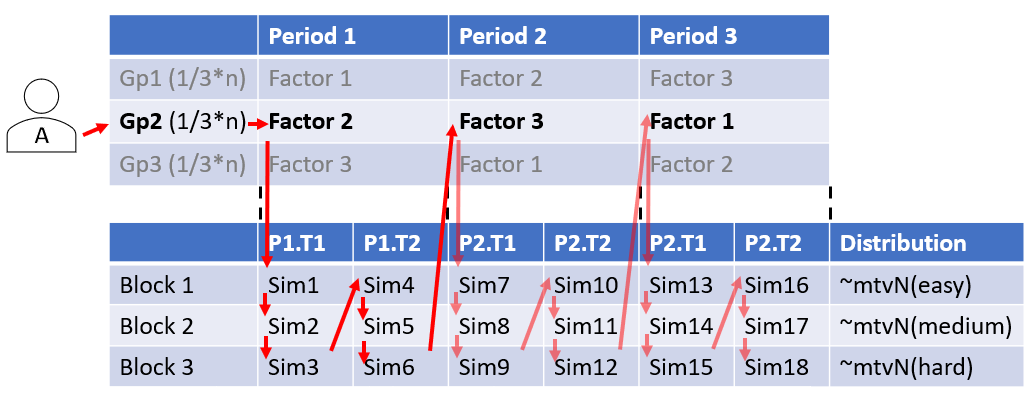
\includegraphics[width=1\linewidth]{./figures/experimental_design_personA} 

}

\caption{Example case. Person 'A' is assigned to group 2, where they will use factor 2 (grand tour) for the first period. They perform 3 block difficulties of task 1 on simulations of increasing difficulty. Then 3 block difficulties of task 2 on unique simulations sampled from the same distributions of increasing difficulty. After this, they proceed to period 2, where they are use factor 3 (manual tour) to perform 3 block difficulties of each task. Lastly, in the third period, they use factor 1 (PCA) to perform the tasks.}\label{fig:designExample}
\end{figure}

\hypertarget{sec:factors}{%
\subsection{Factors}\label{sec:factors}}

We explored performance across three factors. The first factor is
Principal Component Analysis (PCA). The second factor is an animated
walk of interpolation frames between target bases, called a \emph{grand}
tour. The third factor allows for the manual control of the individual
variable's contribution to the projection, performing a \emph{manual}
tour.

All factors are shown as a scatterplot. The basis axes projection was
also illustrated to the left of the plot. They are shown in a unit
circle and show the magnitude and direction each variable contributes to
the projection.

The user interface was kept the same whenever possible, but the control
inputs did change slightly to accommodate the differences between
factors. PCA had 2 side-by-side radio button inputs that select
principal components to display on the x- and y-axes. The manual tour
had the same axes selection, with the addition of a drop-down bar and
slider control. The drop-down selects the variable to manipulate the
contribution of, while the slider controlled the magnitude {[}0-1{]} of
the contribution of that variable on the projection. Performing this
manipulation does require the contributions of the other variables to
change if they are to keep their orthogonal relationship. The grand tour
has no axis or variable inputs and comes precompiled as an animation of
a 15 second showing 90 frames at 6 frames per second. The user can
control the location or play/pause the animation at will. Each frame is
a geodesic interpolation that is close to 0.1 radians away from the
previous frame. These frames will typically include 6 or 7 bases
identified randomly.

\hypertarget{sec:tasks}{%
\subsection{Tasks}\label{sec:tasks}}

Within each factor, participants performed 2 tasks in a fixed order. The
first task asked participants to identify the number of clusters present
in the data. In this task, clusters were unsupervised, where all
observations appeared as black circles. This task does not give insight
to the hypothesis, but rather served as a standard for assessing the
general aptitude for this sort of high dimensional analysis as it was
simpler. In application, linear discriminant analysis (Fisher 1936) or
penalized discriminant analysis (Hastie, Buja, and Tibshirani 1995) are
better suited for classifying such unsupervised data.

The second task is focused on the hypothesis of the study, it asked
participants to identify any/all variables that were very important and
somewhat important for distinguishing a given cluster from the others.
For instance, which variables are very- and somewhat- important for
distinguishing clusters `A' and `B'. This task was supervised by
cluster; observations were assigned shape and (color-blind friendly)
color according to their cluster. A legend identifying cluster by letter
is used for the second task.

\hypertarget{sec:blocks}{%
\subsection{Block difficulty}\label{sec:blocks}}

Participants were randomly assigned to 1 of 3 even groups. Each group
had a different factor order containing all factors. Both tasks were
performed in the same order. Each task had 3 repetitions performed on
new simulations that were drawn from 3 parameterizations in increasing
difficulty. Each participant went through the simulations in the same
order, while their factor order will vary. Fixing block difficulty order
while varying factors should mitigate potential learning bias.

\hypertarget{sec:sim}{%
\subsection{Data simulations}\label{sec:sim}}

The data used for the study were sampled from 4 multivariate normal
distributions. The distributions were parameterized with the number of
clusters, the number of noise variables, and the number of variables.
Each simulation contained either 3 or 4 clusters, with each cluster
containing a random number of observations between 30 and 150. Each
simulation contained 3 or 4 noise variables, which were distributed as
\(~ \mathcal{N}(0, \sigma^2)\). Non-noise variables were distributed
\(~ \mathcal{N}(\mu, \sigma^2)~|~\mu\in \{-9, -8, ... 9\}\) . The
variance-covariance matrix was constrained with non-diagonal elements
selected between -0.1 to 0.6, before being constrained into a positive
definitive matrix.

From the 4 sets of parameterizations, 20 simulations were drawn. The 2
most simple simulations were used during the training section of the
study. All participants were exposed to the same training data sets,
shown in the same order to standardize training. The remaining 18
simulations were drawn such that the remaining 3 parameterizations were
sampled 6 times each. These correspond to the 3 block difficulties of a
given factor and task with increasing difficulty. Referring to the
middle of figure \ref{fig:design}, a participant would perform each
factor-task for 3 block difficulties with increasing difficultly before
proceeding. The next factor-task has 3 new data sets but parameterized
for the same order of increasing difficulty. All participants experience
the same order of simulations while the order of the factor
(visualization) was changed as controlled by a partition into 3 even
groups (top of the same figure).

\hypertarget{sec:response}{%
\subsection{Measures and survey}\label{sec:response}}

The plot display of the first task was limited to 1 minute and 3 minutes
on the second task. Responses we available during and after the timer
was running. The value and time of each response were captured in a
temporary variable that was written to the response table once the user
proceeded to the next page. The number of plot manipulations and
response entries was also captured for each page including training.

After responses for each task were collected, participants were given a
short survey containing questions gauging demographics, experience, and
subjective evaluation of each factor on a 9-point Likert scale. The
questions and possible responses as follows:

\begin{itemize}
\tightlist
\item
  What gender are you? {[}ecline to answer, female, male,
  intergender/other{]}
\item
  What age are you? {[}decline, 19 or younger, 20 to 29, 30 to 39, 40 or
  older{]}
\item
  Is english is your primary language?, {[}decline to answer, English
  first language, English not first language{]}
\item
  What is your highest completed education? {[}decline, highschool,
  undergraduate, honors/masters/mba, doctorate{]}
\item
  I am experienced with data visualization. {[}likert 1-9{]}
\item
  educated in multivariate statistical analysis {[}likert 1-9{]}
\item
  previous familiar with visualization {[}likert 1-9{]} x3 factors
\item
  I found this visualization easy to use. {[}likert 1-9{]} x3 factors
\item
  I felt confident in my answers with this visualization. {[}likert
  1-9{]} x3 factors
\item
  I liked using this visualization. {[}likert 1-9{]} x3 factors
\end{itemize}

Log files were kept where all inputs were tracked with corresponding
timestamps allowing for reproduction if need. Log files, response files,
their analyses, and study application are made publicly available at on
GitHub at
\href{https://github.com/nspyrison/spinifex_study}{github.com/nspyrison/spinifex\_study}

\hypertarget{sec:training}{%
\subsection{Training}\label{sec:training}}

The training was controlled for all participants as much as possible.
All participants received the same written interface instructions and
watched the same training video introducing the methods and the same
task prompts were displayed for their respective tasks. The factor-,
interface-, and task- training took place in a continuous block where
questions were invited. Questions were disallowed once the formal
evaluation section started.

\hypertarget{sec:population}{%
\subsection{Participant population}\label{sec:population}}

A sample of convenience was taken from postgraduate students in the
department of econometrics and business statistics and the faculty of
information technology at Monash University, based in Melbourne,
Australia. Participants were required to have prior knowledge of
multivariate data visualizations.

\hypertarget{sec:results}{%
\section{Results}\label{sec:results}}

\textbf{\#TODO: Need to run study and add results here.}

\hypertarget{sec:spinifex}{%
\section{Accompanying tool: spinifex application}\label{sec:spinifex}}

To accompany this study we have produced a more general use tool to
perform such exploratory analysis of high dimensional data. The R
package, \texttt{spinifex}, \{Spyrison and Cook (2019)\} R package
(version 0.2.0 and up) contains a free, open-source version of a
\texttt{shiny} (Chang et al. 2018) application. The application allows
users to explore their own data with either interactive or predefined
manual tours without the need for any coding. Limited implementations of
grand, little, and local tours are also made available. Data can be
imported in .csv and .rda format, and projections or animations can be
saved as .png, .gif, and .csv formats where applicable. Run the
following R code for help getting started.

\begin{Shaded}
\begin{Highlighting}[]
\KeywordTok{install.packages}\NormalTok{(}\StringTok{"spinifex"}\NormalTok{, }\DataTypeTok{dependencies =} \OtherTok{TRUE}\NormalTok{)}
\NormalTok{spinifex}\OperatorTok{::}\KeywordTok{run_app}\NormalTok{(}\StringTok{"intro"}\NormalTok{)}
\NormalTok{spinifex}\OperatorTok{::}\KeywordTok{run_app}\NormalTok{(}\StringTok{"primary"}\NormalTok{)}
\end{Highlighting}
\end{Shaded}

\hypertarget{sec:discussion}{%
\section{Discussion}\label{sec:discussion}}

\hypertarget{sec:acknowledgments}{%
\section{Acknowledgments}\label{sec:acknowledgments}}

This article was created in R (R Core Team 2019), using \texttt{knitr}
(Xie 2014) and \texttt{rmarkdown} (Xie, Allaire, and Grolemund 2018),
with code generating the examples inline. The source files for this
article be found at
\href{https://github.com/nspyrison/spinifex_paper/}{github.com/nspyrison/spinifex\_study/}.
The source code for the \texttt{spinifex} package and accompanying shiny
application can be found at
\href{https://github.com/nspyrison/spinifex/}{github.com/nspyrison/spinifex/}.

\hypertarget{sec:bib}{%
\section*{Bibliography}\label{sec:bib}}
\addcontentsline{toc}{section}{Bibliography}

\hypertarget{refs}{}
\leavevmode\hypertarget{ref-anscombe_graphs_1973}{}%
Anscombe, F. J. 1973. ``Graphs in Statistical Analysis.'' \emph{The
American Statistician} 27 (1): 17--21.
\url{https://doi.org/10.2307/2682899}.

\leavevmode\hypertarget{ref-asimov_grand_1985}{}%
Asimov, Daniel. 1985. ``The Grand Tour: A Tool for Viewing
Multidimensional Data.'' \emph{SIAM Journal on Scientific and
Statistical Computing} 6 (1): 128--43.
\url{https://doi.org/https://doi.org/10.1137/0906011}.

\leavevmode\hypertarget{ref-chambers_graphical_1983}{}%
Chambers, J. M., W. S. Cleveland, B. Kleiner, and P. A. Tukey. 1983.
``Graphical Methods for Data Analysis.''

\leavevmode\hypertarget{ref-chang_shiny:_2018}{}%
Chang, Winston, Joe Cheng, J. J. Allaire, Yihui Xie, and Jonathan
McPherson. 2018. \emph{Shiny: Web Application Framework for R}.
\url{https://CRAN.R-project.org/package=shiny}.

\leavevmode\hypertarget{ref-cook_manual_1997}{}%
Cook, Dianne, and Andreas Buja. 1997. ``Manual Controls for
High-Dimensional Data Projections.'' \emph{Journal of Computational and
Graphical Statistics} 6 (4): 464--80.
\url{https://doi.org/10.2307/1390747}.

\leavevmode\hypertarget{ref-fisher_use_1936}{}%
Fisher, Ronald A. 1936. ``The Use of Multiple Measurements in Taxonomic
Problems.'' \emph{Annals of Eugenics} 7 (2): 179--88.
\url{https://doi.org/10.1111/j.1469-1809.1936.tb02137.x}.

\leavevmode\hypertarget{ref-hastie_penalized_1995}{}%
Hastie, Trevor, Andreas Buja, and Robert Tibshirani. 1995. ``Penalized
Discriminant Analysis.'' \emph{The Annals of Statistics}, 73--102.

\leavevmode\hypertarget{ref-karwowski_international_2006}{}%
Karwowski, Waldemar. 2006. \emph{International Encyclopedia of
Ergonomics and Human Factors, -3 Volume Set}. CRC Press.

\leavevmode\hypertarget{ref-kohonen_self-organizing_1990}{}%
Kohonen, Teuvo. 1990. ``The Self-Organizing Map.'' \emph{Proceedings of
the IEEE} 78 (9): 1464--80.

\leavevmode\hypertarget{ref-maaten_visualizing_2008}{}%
Maaten, Laurens van der, and Geoffrey Hinton. 2008. ``Visualizing Data
Using T-SNE.'' \emph{Journal of Machine Learning Research} 9 (Nov):
2579--2605.

\leavevmode\hypertarget{ref-matejka_same_2017}{}%
Matejka, Justin, and George Fitzmaurice. 2017. ``Same Stats, Different
Graphs: Generating Datasets with Varied Appearance and Identical
Statistics Through Simulated Annealing.'' In \emph{Proceedings of the
2017 CHI Conference on Human Factors in Computing Systems - CHI '17},
1290--4. Denver, Colorado, USA: ACM Press.
\url{https://doi.org/10.1145/3025453.3025912}.

\leavevmode\hypertarget{ref-pearson_liii._1901}{}%
Pearson, Karl. 1901. ``LIII. On Lines and Planes of Closest Fit to
Systems of Points in Space.'' \emph{The London, Edinburgh, and Dublin
Philosophical Magazine and Journal of Science} 2 (11): 559--72.

\leavevmode\hypertarget{ref-r_core_team_r:_2019}{}%
R Core Team. 2019. \emph{R: A Language and Environment for Statistical
Computing}. Vienna, Austria: R Foundation for Statistical Computing.
\url{https://www.R-project.org/}.

\leavevmode\hypertarget{ref-spyrison_spinifex_2019}{}%
Spyrison, Nicholas S., and Dianne Cook. 2019. \emph{Spinifex: Manual
Tours, Manual Control of Dynamic Projections of Numeric Multivariate
Data} (version 0.1.0.9000).
\url{https://github.com/nspyrison/spinifex/}.

\leavevmode\hypertarget{ref-tukey_exploratory_1977}{}%
Tukey, John W. 1977. \emph{Exploratory Data Analysis}. Vol. 32. Pearson.

\leavevmode\hypertarget{ref-stodden_knitr:_2014}{}%
Xie, Yihui. 2014. ``Knitr: A Comprehensive Tool for Reproducible
Research in R.'' In \emph{Implementing Reproducible Computational
Research}, edited by Victoria Stodden, Friedrich Leisch, and Roger D.
Peng. Chapman; Hall/CRC.
\url{http://www.crcpress.com/product/isbn/9781466561595}.

\leavevmode\hypertarget{ref-xie_r_2018}{}%
Xie, Yihui, J. J. Allaire, and Garrett Grolemund. 2018. \emph{R
Markdown: The Definitive Guide}. Boca Raton, Florida: Chapman; Hall/CRC.
\url{https://bookdown.org/yihui/rmarkdown}.

\end{document}
